% template.tex, dated April 5 2013
% This is a template file for Annual Reviews 1 column Journals
%
% Compilation using ar-1col.cls' - version 1.0, Aptara Inc.
% (c) 2013 AR
%
% Steps to compile: latex latex latex
%
% For tracking purposes => this is v1.0 - Apr. 2013

\documentclass[letterpaper,draft]{ar-1col}
\usepackage[numbers]{natbib}
\usepackage[left=35mm,top=26mm,right=26mm,bottom=15mm]{geometry}




\usepackage[american]{babel}
% \usepackage{amsmath}
% \usepackage[version=3]{mhchem} 
% % \usepackage{fixltx2e}
% % \usepackage{refcount}
% % \usepackage{siunitx}
% % \usepackage{lastpage}
% % \usepackage{textcomp}
% \usepackage{mathtools}
% 
% \usepackage{xfrac}
\usepackage{lmodern}
\usepackage[hidelinks]{hyperref}
% % \usepackage{cool}
% % \usepackage{cancel}
% % \usepackage{microtype}
% \usepackage{listings}
% % \usepackage{mcode}
\usepackage [autostyle, english = american]{csquotes}
% % \usepackage{longtable}
% % \usepackage{subcaption}
% \usepackage{booktabs,siunitx}
% \usepackage{gensymb}
% \usepackage[normalem]{ulem}

% \usepackage{mathtools, cuted}
\usepackage{wrapfig}


% \usepackage[usenames,dvipsnames,svgnames,table]{xcolor}
% \usepackage{color}

% \usepackage[colorinlistoftodos]{todonotes}

% \usepackage[section]{placeins}
% \usepackage{multirow}

% \usepackage{lineno}

\usepackage{graphicx}% Include figure files
% \usepackage{dcolumn}% Align table columns on decimal point



% Sin and Cos with auto-parentheses 
\newcommand{\sinp}[1]{\sin{\left( #1\right)}}
\newcommand{\cosp}[1]{\cos{\left( #1\right)}}
\newcommand{\expp}[1]{\exp{\left( #1\right)}}
\newcommand{\sinhp}[1]{\sinh{\left( #1\right)}}
\newcommand{\lnp}[1]{\ln{\left( #1\right)}}
\newcommand{\pp}[1]{\left( #1\right)}
\newcommand{\sci}[2]{ #1 \cdot 10^{#2}\ }
\newcommand{\angstrom}{\mbox{\normalfont\AA}}
\newcommand{\norm}[1]{\lVert #1 \rVert}

\newcommand{\textred}[1]{\textcolor{red}{ #1}}
\newcommand{\redactedit}[1]{\textcolor{blue}{ \sout{#1}}}

\newcommand{\cmmnt}[1]{}


\newcommand{\colornote}[1]{\textcolor{red}{ COMMENT\large\footnote{\textcolor{red}{#1}}}}

\newcommand{\comment}[1]{\todo[color=blue!20!white,inline]{ASV: #1}} 

\newcommand{\etal}{\emph{et\,al.}} 


% Tweak sim for better inline text tilde
\newcommand{\mytilde}{\raisebox{0.5ex}{\texttildelow}}
% \newcommand{\mytilde}{\raise.17ex\hbox{$\scriptstyle‌​\sim$}}

% \sisetup{separate-uncertainty=true,table-space-text-post = *}

\newcommand{\minitab}[2][l]{\begin{tabular}{#1}#2\end{tabular}}

% \newcounter{subfigure}[figure]

\newcommand{\subfigimg}[4][,]{%
  \setbox1=\hbox{\noindent\includegraphics[#1]{#3}}% Store image in box
  \leavevmode\rlap{\usebox1}% Print image
  \rlap{\hspace*{#4pt}\raisebox{\dimexpr\ht1-2\baselineskip}{#2}}% Print label
  \phantom{\usebox1}% Insert appropriate spcing
}
% \subfigimg[scale=0.59]{a)}{./figures/after_minimization_plot_alt.pdf}{80pt}

% \usepackage[style=base]{caption}
% \usepackage{subfig}
% Remove a), b), etc labels from subfigs
% \captionsetup[subfigure]{labelformat=empty}
% \captionsetup{style=base} 

% Sick of fighting siunitx - consistent text micro symbol
% DO NOT uncomment this!!! or else broken unicode (Âţ)
% \sisetup{math-micro=\text{µ},text-micro=µ}
% \si\micro
\newcommand{\mmicro}{\si\micro} 

% \usepackage{adjustbox}


% \makeatletter
% % Make common definition of mean
% \newcommand*\mean[1]{\overline{#1\raisebox{3mm}{}}}
% 
% \makeatother

\hyphenation{gamma-rays}

% \setcounter{secnumdepth}{4}


% 
% 
% 
% Journal template info
% 
% 
% 
% 
% 
% 
% 
% 



% Metadata Information
\jname{Xxxx. Xxx. Xxx. Xxx.}
\jvol{AA}
\jyear{YYYY}
\doi{10.1146/((please add article doi))}


% Document starts
\begin{document}

% Page header
\markboth{Bernstein et al.}{Our Future Nuclear Data Needs}

% Title
\title{Our Future Nuclear Data Needs}


%Authors, affiliations address.
\author{Lee A. Bernstein$^{1,2}$, David A. Brown$^3$, \\Arjan J. Koning$^4$, Brad T. Rearden$^5$,  \\Catherine E. Romano$^5$, Alejandro A. Sonzogni$^3$, Andrew S. Voyles$^{1,2}$, and Walid  Younes$^6$
\affil{$^1$Nuclear Science Division, Lawrence Berkeley National Laboratory,  Berkeley, CA 94720, USA; email: labernstein@lbl.gov}
\affil{$^2$Department of Nuclear Engineering, University of California, Berkeley,  Berkeley, CA 94720, USA}
\affil{$^3$Brookhaven National Laboratory, Upton, NY 11973, USA}
\affil{$^4$Arjan's affiliations}
\affil{$^5$Oak Ridge National Laboratory, Oak Ridge, TN 37830, USA}
\affil{$^6$Lawrence Livermore National Laboratory,  Livermore, CA 94550, USA}}

%Abstract
\begin{abstract}
A well-established knowledge of nuclear phenomena including fission, reaction cross sections, and structure/decay properties, is critical for applications ranging from the design of new reactors, to non-proliferation, to the production of radioisotopes for the diagnosis and treatment of illness.  However, the lack of a well-quantified, predictive theoretical capability means that most nuclear observables must be measured directly in order to “calibrate” empirical models, which, in turn, provide the data needed for these applications.  In many cases there is either a lack of the data needed to guide the models, or the results of the different measurements are discrepant.  This has led to the development of evaluation methodologies to provide recommended values and uncertainties.  In this article we present the nuclear data evaluation process and the international community that carries it out.  We then discuss new measurements and improved theory and/or modeling needed to address future challenges in applied nuclear science. 
\end{abstract}

%Keywords, etc.
\begin{keywords}
keywords, separated by comma, no full stop, lowercase
\end{keywords}
\maketitle

%Table of Contents
\tableofcontents


% Heading 1
\section{INTRODUCTION}

\subsection{The Two Faces of Nuclear Data}


Low-energy nuclear science (LENS) \enquote{straddles the fence} between curiosity- and application-driven pursuits.  On the curiosity-driven side, low-energy ($E_x <$ 1--4 MeV) nuclear structure offers a unique laboratory to examine the interplay between single-particle and collective behavior and to explore the transition from quantum to continuum behavior in a mesoscopic setting. LENS also plays an important role in nuclear astrophysics, improving models of stellar energy generation and allowing isotopic abundances to be used to inform models of the astrophysical environments where heavy nuclei are formed.  On the applied side, a well-quantified knowledge of low-lying nuclear structure and reactions is needed to model energy generation and isotope production for medical and industrial uses and for the national security and counter-proliferation communities.   

One hallmark of LENS is that most theoretical descriptions are descriptive rather than rigorously predictive at the level of accuracy and over the entire range of energies etc. needed for real world applications.  As a result, targeted measurements coupled to a data evaluation process are used to produce databases of recommended values that can be employed by the user communities.  The evaluation processes range from close adherence to experimental results in the case of low energy nuclear structure and decay data, to experiment-guided modeling in the case of nuclear reactions. This work is carried out by subject matter experts who usually come from the field utilizing the data who spend many years studying under experienced evaluators in order to develop the highly-specialized skills they need.  

This manuscript will start with a description of the nuclear data evaluation process, and the organizations organization that carry it out.  It will then describe ways to improve the modeling of (n,x) reactions on nuclides important for applications.  Following this will be a discussion of needs for specific applications including national security/non-proliferation, medical isotope production and nuclear energy.  It will end with a discussion of the future of nuclear data featuring  a new, Nuclear Data Interagency Working Group that that is formulating a national nuclear data plan to address high-priority needs for applied nuclear science and technology.   


\subsection{The Nuclear Data Pipeline}

Before diving into the data needs, it is instructive to understand the \enquote{Nuclear Data Pipeline} that takes experimental or theoretical results and prepares them for use in applications.  This process is illustrated in \autoref{fig:pipeline} and is roughly grouped into four steps: 1) compilation, 2) evaluation, 3) processing, and 4) validation.  This process ends with the users and their application, but actually begins with the performance of carefully-designed measurements with well-defined uncertainties.  Given this, it behooves those funding or performing the original experiment to understand the entire nuclear data workflow in order to ensure that new results find their way to the intended user.  For example, if a new result forces changes to data formats (step 2) or processing (step 3) or to application codes (step 4 \& eventual user), this fact should be considered when developing a new activity.

The first step in the Pipeline is compilation and it begins with potentially the most important database: Nuclear Science References (NSR) \cite{NSR}.  NSR contains references to published works from major LENS journals as well as internal reports from labs throughout the world and serves as the start point for the data evaluation process. Descriptive keywords are assigned to these articles by individuals with LENS backgrounds, enabling the use of this information in later portions of the evaluation process.   



\begin{wrapfigure}{r}{0.4\textwidth}
\centering
\includegraphics[width=0.4\textwidth]{pipeline_cropped.pdf}
\caption{\label{fig:pipeline}The nuclear data pipeline.}
\end{wrapfigure}



Following this, the data from the primary references contained in NSR, including both mean values and uncertainties, are extracted in numerical form and compiled into one of two databases depending on whether the data is primarily regarding nuclear structure and decay or nuclear reaction data.   This step may also include tracking down unpublished data from original sources before that data is lost.

The nuclear structure compilation database is called the Experimental Unevaluated Nuclear Data List (XUNDL) \cite{XUN}.   The nuclear data in XUNDL is organized by nuclide, meaning that a single publication could lead to the production of more than one XUNDL dataset.  Each XUNDL dataset is treated as a “stand-alone” work and is not required to agree with existing, evaluated nuclear data for the nuclide it concerns.  However, during XUNDL compilation basic consistency checks are performed and any internal inconsistencies are pointed out to the author to allow them be reconciled in the database.  XUNDL is used by both nuclear structure evaluators to aid in their work and by nuclear structure researchers as a quick way to get access to data from current publications in order to guide their own research. 

The nuclear reaction compilation database is referred to as Experimental Nuclear Reaction Data library (EXFOR) \cite{EXF}.  This includes not only reaction cross sections, but also related data such as fission yields, resonance integrals, polarization data and more.  Given the wide range of data types present in EXFOR there is significantly less error checking than what is performed during in XUNDL compilation.  However, an online visualization tool is provided to allow users to plot and manipulate the data. EXFOR is used by both nuclear reaction evaluators and the nuclear reaction research and application community. 

The next step in the process is evaluation itself.  In the case of nuclear structure data this involves reconciling multiple types data sets (e.g., prompt gamma and particle spectra, decay data etc.) and deriving a recommended set of adopted values.  This data forms the basis of the Evaluated Nuclear Structure Data File (ENSDF) \cite{tepel1984ensdf}.  While most of the ENSDF evaluation is performed in the US, there is a significant and growing component coming from evaluators throughout the world.  The governing body that determines the rules for the evaluation process is the Nuclear Structure and Decay Data Network administered by the International Atomic Energy Agency (IAEA-NSDD).  

In the case of nuclear reaction data, the process is markedly different.  The data from EXFOR is used to guide a physics-based model calculation through a variety of variance minimization procedures, resulting in best estimates of mean values and their uncertainties, including covariances, which are put into the Evaluated Nuclear Data File \cite{Chadwick2011}.  Most of the effort put into the production of ENDF is provided by applications-oriented users due to its importance to national security, international counter-proliferation and nuclear energy.  A consequence of this application focus is that the vast majority of the data in ENDF concerns neutron-induced reactions at either thermal (25 meV), fast fission or 14.1 MeV.  This has profound implications for isotope production since many of the nuclides are produced through charged-particle induced reactions.  

While ENSDF and ENDF contain a vast quantity of nuclear data, there are significant amounts of nuclear data that are either not contained in them because they “fall between” nuclear structure and nuclear reactions, or they are present in a format that is not well-suited to their use in applications.  Examples of this include the recently updated Atlas of Neutron Resonances \cite{Mug18} which contains neutron capture resonance widths, centroids and cross sections and the Evaluated Gamma Activation File of (EGAF) capture gamma-rays \cite{Fir15} and the Atlas of Inelastic Scattering of Reactor Fast Neutron \cite{Hur18}.  Another very important nuclear data resource for applications is the Reference Input Parameter Library (RIPL) \cite{Capote2009} which contains both discrete (distilled from ENSDF) and continuous (Nuclear Level Densities and Gamma-strength function) nuclear structure data needed for accurate reaction modeling.  
	
Evaluations in hand, we must now process the data into a form suitable for use in a particular application.  This is a surprisingly non-trivial part of the process, requiring a deep knowledge of the physics used in the evaluation process, the formatting limitations of intermediate data formats, and the capabilities of downstream codes that will use the nuclear data.  Processing is also needed for the validation of nuclear reaction data using the integral benchmarks described below.  Another role of processing is in the creation of application-specific databases, such as the Medical Internal Radiation Dose (MIRD) \cite{MIRD} database used to guide medical treatment and diagnosis.  

The final step in the Pipeline is validation.  In this step, we use user codes and user-defined problems to validate that the data performs as expected.  The class of user problems we most rely on are so-called “integral benchmark” data that depend on many different types of data including cross sections and emitted particle spectra and are also extremely precisely known.  The canonical example of such a benchmark is a critical assembly, where the ratio of neutron production to neuron loss (k­eff) is known to several significant figures.  However, there are many other kinds of integral benchmarks used to test neutron interaction data alone, including reaction rate measurements and 14 MeV and fission spectrum transmission experiments, and many more for other forms of nuclear data.

There are multiple ways to interact with the nuclear data evaluation process along the way, including through web interfaces hosted by the National Nuclear Data Center \cite{NNDC} and the IAEA Nuclear Data Section \cite{IAEA-NDS}, a smartphone based application \cite{IAEA-APP} and publication in peer-reviewed journals including Nuclear Data Sheets \cite{NDS} and Atomic Data and Nuclear Data Tables \cite{ATNDT}.  

Many different government agencies support nuclear data evaluation activities, including several components of the Department of Energy National Nuclear Security Agency (DOE-NNSA) and the National Criticality Safety Program (NCSP).  However, the primary domestic organization responsible for organizing the evaluation process is US Nuclear Data Program (USNDP) in the DOE Nuclear Physics office (DOE-NP).  The USNDP is headquartered at the National Nuclear Data Center at Brookhaven National Lab and includes centers at Argonne, Oak Ridge, Los Alamos and Lawrence Livermore National Labs, as well as joint lab/university programs at North Carolina State University/Triangle University Nuclear Lab, Michigan State University/National Superconducting Cyclotron Lab and the University of California/Lawrence Berkeley National Laboratory.   


\subsection{International Collaboration}

Much of the work of nuclear data evaluation takes place as a part of international collaborations covered under the Organization of Economic Cooperation and Development’s Nuclear Energy Agency (NEA) and the International Atomic Energy Agency (IAEA).  The Nuclear Energy Agency (NEA) addresses the nuclear technology interests of its 33 member states and, in the area of nuclear data, the Working Party on Evaluation Coordination (WPEC) is the main forum for collaborative effort between the nuclear data library projects from the NEA countries, namely ENDF/B (United States), JENDL (Japan), JEFF (NEA), TENDL (Europe), BROND (Russia) as well as the non-OECD file project CENDL (China).

A powerful instrument of WPEC to drive progress in nuclear data is the so-called Subgroup (SG): members of WPEC identify a common area in nuclear data that requires improvement, and if enough support from the various data library projects is present, a Subgroup is formed.  Subgroups typically operate on a 3-5 year time frame. Recent successful examples of WPEC subgroups, which specific relevance to the US, are large-scale horizontal efforts like CIELO (SG40), on worldwide nuclear data evaluation for the most important fission energy related materials. The CIELO initiative has for example led to new ENDF/B-VIII.0 evaluations for 235,238U, 56Fe and 16O among others, and the Generalized Nuclear Database Structure (GNDS) format (SG38) \cite{SG38}, or more specific efforts like covariance adjustment for improvement of nuclear data files (SG39) \cite{SG39}. 

WPEC also hosts long-term Expert Groups, and current groups are working on the development of the Generalized Nuclear Database Structure (GNDS) format, to provide a data library interface between nuclear physics and applications more modern than the ENDF-6 format, and the High-Priority Request List which assembles the most important nuclear data requests from applications in a unified format, to stimulate experimentalists and evaluators to provide these data. A full list of past and current subgroups of WPEC is available at Ref. \cite{WPEC}.
 
The International Atomic Energy Agency (IAEA) covers the interests of its 170 member states. The main task of the IAEA Nuclear Data Section is to provide fundamental nuclear data bases for basic and applied use, with data originating from experiments and theoretical simulations and covering both nuclear structure and nuclear reaction data.  An important collaboration coordinated by the IAEA is the Nuclear Reaction Data Center Network, which is responsible for keeping the EXFOR database of experimental nuclear reaction data up to date. NNDC is responsible for the US input to the database.  

In addition, the IAEA organizes Coordinated Research Projects (CRP) and technical meetings as instruments to align international nuclear data efforts towards the production of validated databases ready for applied use.  Examples of recent and current CRP's include a 2018 venture centered on nuclear data for primary radiation damage has been completed, an ongoing effort to improve nuclear model parameters for fission reaction calculations by modern nuclear model codes such as EMPIRE \cite{Her07}, CCONE \cite{Iwa16}, COH3 \cite{Kaw10} and TALYS \cite{Kon08} is ongoing, and an effort to create a first-ever evaluated database of radiative strength.  In 2019, a CRP on fission yields will start which aims to produce updated fission yield libraries for the major actinides to respond to requests from reactor technology, safeguards and non-proliferation.

Nuclear data evaluations of neutron-induced reactions for fission applications are covered by the International Nuclear Data Evaluation Network (INDEN), an IAEA initiative which continues the CIELO efforts of the NEA for differential nuclear data developments, and evaluations, for the most important materials relevant for fission technology.  Other long term projects are the nuclear structure and decay data network NSDD, nuclear data for medical isotope production, with emphasis on data needs for monitor reactions and accelerator, neutron standards and the Fusion Evaluated Nuclear Data Library FENDL.

\section{IMPROVED (N,X) REACTION MODELING: A CROSSCUTTING NEED}

Accurate, physics-based modeling of neutron-induced reactions, particularly on the “Big 3” (235,238U and 239Pu) are key to virtually all nuclear science and technology applications.  While a great deal of effort has been made to improve (n,f) data, a fundamental understanding of this most important of reaction mechanisms remain elusive.  Furthermore, since fission leads to the production of neutrons with energies up to several MeV, elastic and inelastic scattering also play a critical role.  Unfortunately, efforts to improve neutron scattering data has tended to “take a back seat” to fission due to a deficit of high-quality experimental data.  Lastly, while all modeling of (n,x) reactions requires a good understanding of unbound nuclear states populated in (n,x) reactions, it remains one of the least understood topics in LENS.  In this section we explore all three of these topics these “crosscutting” topics and present plans to improve them.  

\subsection{A Deeper Understanding of Fission}

Not all fission data needed in nuclear physics applications can be readily measured in the laboratory. In many cases, the targets may be too-short lived, the analysis might yield unacceptably large uncertainties, or separate measurements of the same quantity may produce discrepant results. As with other reaction data, fission evaluation proceeds through the use of a model designed to reproduce the data as closely as possible.  However, in the case of fission, we still lack a predictive theoretical framework to match all types of measured data within experimental errors. A truly predictive theory of fission will require advances in theoretical techniques and computational machinery, along with improved experimental data.

For fission theory, we can make a distinction in practice between description of the fission process up to scission (pre-scission physics), and the events that follow scission (post-scission physics). Eventually, one could envision a comprehensive model that accurately follows the entire fission process from the formation of the parent nucleus to the last decays of the final product nuclei within a single internally consistent theoretical framework. Such a model is not yet feasible so different physics models are used to treat pre- and post-scission processes. A wide range of theoretical approaches have been developed since the late 1930's to describe pre-scission physics, including scission-point models \cite{Wil76,Lem15}, microscopic-macroscopic models \cite{Moller2015} with random-walk dynamics \cite{Wa17}, Langevin dynamics \cite{Sie17}, Time-dependent Hartree-Fock and Hartree-Fock-Bogoliubov theory \cite{Koo76,Neg78,Tan15,God16}, the time-dependent superfluid local density approximation \cite{Ste11,Bul13,Ste15,Bul16}, and the time-dependent generator-coordinate method \cite{Ber91,Gou05,Rei16}.Several models have also been developed to describe post-scission physics and built into computer codes, such as GEF \cite{Sch16}, FIFRELIN \cite{Lit15}, CGMF \cite{Kaw10}, and FREYA \cite{Ran09,Ver18}.

The division between pre- and post-scission physics in modeling efforts suggests a corresponding division in nuclear data needs to improve our understanding of the fission process. Post-scission observables are generally easier to measure, and include the properties of fission fragments and products and of the neutrons and gamma rays they emit.  Recently, Bertsch et al. \cite{Ber15} have suggested a subset of fission data that tend to have relatively small uncertainties and could therefore be used to test and validate fission models. These data consist of fission barriers, fragment mass distributions, fragment total kinetic energies, spontaneous-fission lifetimes, and fission isomer excitation energies. In addition to these quantities, the angular distribution of fission fragments can also provide useful information about the angular momentum of the fissioning nucleus and further constrain model calculations. 

In addition to standard experiments looking at individual fission properties, multi-parameter measurements that give a comprehensive view of a fission event should be pursued as facilities and detectors improve. Ideally, a multi-parameter experiment would record all possible fission observables (e.g., fragment charge, mass, and energy distributions as well as neutron and gamma spectra and multiplicities) on an event-by-event basis, thereby making it possible to reconstruct the state of the nucleus at scission. In practice, each additional observable reduces statistics, making such measurements exceedingly challenging. Finally, there are experimental measurements that directly probe the pre-scission dynamics of the fission process although they carry large uncertainties and suffer from various ambiguities and limitations. These include measurements of scission neutrons \cite{Pe09}, fission time scales \cite{Jac09}, and muon-induced fission \cite{Mar80}. Probes of pre-scission physics can provide unique insights into the details of the fission process, and are therefore extremely valuable to fission theory.

Both pre-scission and post-scission theory and data will be needed to reach a satisfactory understanding of the fission process, and thereby make reliable predictions of nuclear quantities that cannot be measured in the laboratory. Pre-scission models can provide input to post-scission models wherever the data are lacking, and post-scission models can be used to improve pre-scission calculations using a wealth of available experimental data. The ultimate goal for theorists, a comprehensive description of fission starting from protons, neutrons, and their interactions that provides accurate values for all fission data of interest, remains elusive.  Many questions about the fission process remain open, such as: how the initial partition of energy between kinetic and internal excitation occurs, what the relevant collective and single-particle degrees of freedom are near scission, and how they evolve and couple throughout the process? Lastly, how can we best quantify uncertainties (both epistemic and aleatory) in fission calculations?

%Heading 1
\section{FIRST-LEVEL HEADING}
This is dummy text. 
% Heading 2
\subsection{Second-Level Heading}
This is dummy text. This is dummy text. This is dummy text. This is dummy text.

% Heading 3
\subsubsection{Third-Level Heading}
This is dummy text. This is dummy text. This is dummy text. This is dummy text. 

% Heading 4
\paragraph{Fourth-Level Heading} Fourth-level headings are placed as part of the paragraph.

%Example of a Figure
% \section{ELEMENTS\ OF\ THE\ MANUSCRIPT} 
% \subsection{Figures}Figures should be cited in the main text in chronological order. This is dummy text with a citation to the first figure (\textbf{Figure \ref{fig1}}). Citations to \textbf{Figure \ref{fig1}} (and other figures) will be bold. 
% 
% \begin{figure}[h]
% 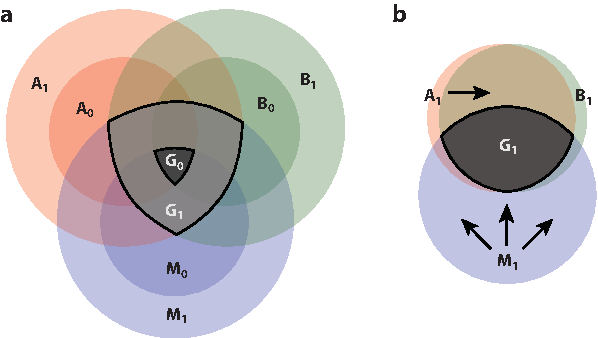
\includegraphics[width=3in]{SampleFigure.pdf}
% \caption{Figure caption with descriptions of parts a and b}
% \label{fig1}
% \end{figure}
% 
% % Example of a Table
% \subsection{Tables} Tables should also be cited in the main text in chronological order (\textbf {Table \ref{tab1}}).
% 
% \begin{table}[h]
% \tabcolsep7.5pt
% \caption{Table caption}
% \label{tab1}
% \begin{center}
% \begin{tabular}{@{}l|c|c|c|c@{}}
% \hline
% Head 1 &&&&Head 5\\
% {(}units)$^{\rm a}$ &Head 2 &Head 3 &Head 4 &{(}units)\\
% \hline
% Column 1 &Column 2 &Column3$^{\rm b}$ &Column4 &Column\\
% Column 1 &Column 2 &Column3 &Column4 &Column\\
% Column 1 &Column 2 &Column3 &Column4 &Column\\
% Column 1 &Column 2 &Column3 &Column4 &Column\\
% \hline
% \end{tabular}
% \end{center}
% \begin{tabnote}
% $^{\rm a}$Table footnote; $^{\rm b}$second table footnote.
% \end{tabnote}
% \end{table}
% 
% % Example of lists
% \subsection{Lists and Extracts} Here is an example of a numbered list:
% % \begin{enumerate}
% % \item List entry number 1,
% % \item List entry number 2,
% % \item List entry number 3,\item List entry number 4, and
% % \item List entry number 5.
% % \end{enumerate}
% 
% % Here is an example of a extract.
% % \begin{extract}
% % This is an example text of quote or extract.
% % This is an example text of quote or extract.
% % \end{extract}
% 
% \subsection{Sidebars and Margin Notes}
% % Margin Note
% \begin{marginnote}[]
% \entry{Term A}{definition}
% \entry{Term B}{definition}
% \entry{Term C}{defintion}
% \end{marginnote}
% 
% \begin{textbox}[h]\section{SIDEBARS}
% Sidebar text goes here.
% \subsection{Sidebar Second-Level Heading}
% More text goes here.\subsubsection{Sidebar third-level heading}
% Text goes here.\end{textbox}
% 
% 
% 
% \subsection{Equations}
% % Example of a single-line equation
% \begin{equation}
% a = b \ {\rm ((Single\ Equation\ Numbered))}
% \end{equation}
% %Example of multiple-line equation
% Equations can also be multiple lines as shown in Equations 2 and 3.
% \begin{eqnarray}
% c = 0 \ {\rm ((Multiple\  Lines, \ Numbered))}\\
% ac = 0 \ {\rm ((Multiple \ Lines, \ Numbered))}
% \end{eqnarray}
% 
% % Summary Points
% \begin{summary}[SUMMARY POINTS]
% \begin{enumerate}
% \item Summary point 1. These should be full sentences.
% \item Summary point 2. These should be full sentences.
% \item Summary point 3. These should be full sentences.
% \item Summary point 4. These should be full sentences.
% \end{enumerate}
% \end{summary}
% 
% % Future Issues
% \begin{issues}[FUTURE ISSUES]
% \begin{enumerate}
% \item Future issue 1. These should be full sentences.
% \item Future issue 2. These should be full sentences.
% \item Future issue 3. These should be full sentences.
% \item Future issue 4. These should be full sentences.
% \end{enumerate}
% \end{issues}

%Disclosure
\section*{DISCLOSURE STATEMENT}
If the authors have noting to disclose, the following statement will be used: The authors are not aware of any affiliations, memberships, funding, or financial holdings that
might be perceived as affecting the objectivity of this review. 

% Acknowledgements
\section*{ACKNOWLEDGMENTS}
Acknowledgements, general annotations, funding.

% References
%
% Margin notes within bibliography
\section*{LITERATURE\ CITED}

\bibliographystyle{ar-style5}

\bibliography{../../library}




 

% \end{thebibliography}


\end{document}
